% Defense slide 7: the contraction as repeated application of the transfer
% matrix, <b_L| E E ... E |b_R>, contracted along SPACE.
% The boundary vectors b_L, b_R are NOT columns of the network: they are
% arbitrary (in practice random) temporal MPS, drawn as separate orange
% chains -- the power method converges them to the dominant pair <L|, |R>.
% Network conventions follow thesis/imgs/echo_strip.tex.
\documentclass[tikz,border=3pt]{standalone}
\usepackage{amsmath,amssymb,braket}
\usetikzlibrary{arrows.meta}

\newcommand{\NX}{4}   % network columns 0..4 (five E columns)
\newcommand{\DX}{1.10}
\newcommand{\DY}{0.60}

\definecolor{tnbulk}{RGB}{86,196,229}
\definecolor{tncool}{RGB}{240,224,178}
\definecolor{tnbox}{RGB}{40,130,70}
\definecolor{tnbnd}{RGB}{196,98,22}

\begin{document}
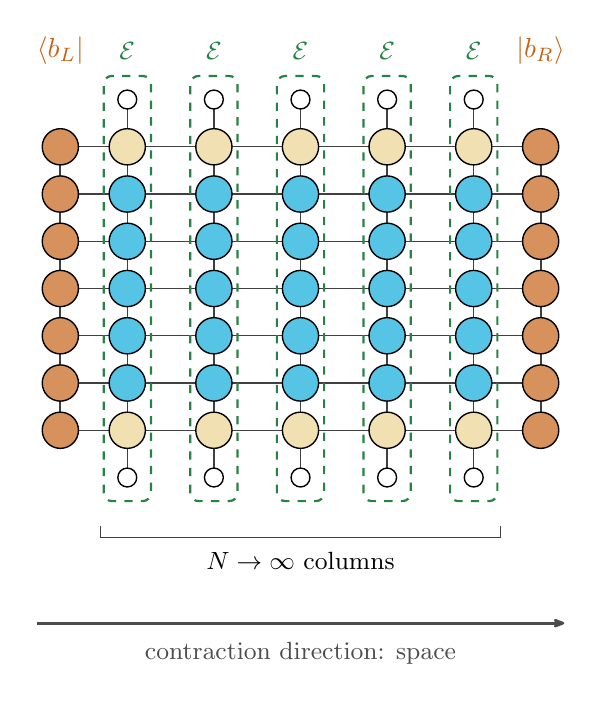
\begin{tikzpicture}[
    >={Stealth[round,length=2.0mm]},
    leg/.style={draw=black!75, line width=0.45pt},
    W/.style={circle, draw=black, fill=tnbulk, line width=0.5pt, minimum size=4.6mm, inner sep=0pt},
    B/.style={circle, draw=black, fill=tncool, line width=0.5pt, minimum size=4.6mm, inner sep=0pt},
    P/.style={circle, draw=black, fill=white, line width=0.5pt, minimum size=2.4mm, inner sep=0pt},
    V/.style={circle, draw=black, fill=tnbnd!70, line width=0.5pt, minimum size=4.6mm, inner sep=0pt},
    vbox/.style={draw=tnbox, dashed, line width=0.8pt, rounded corners=3pt},
    tag/.style={font=\small},
  ]

  %% the network: rows = time, columns = space (every column is E)
  \foreach \i in {0,...,\NX} { \draw[leg] (\i*\DX,0) -- (\i*\DX,{8*\DY}); }
  % horizontal legs extend past the outer columns to reach the boundary chains
  \foreach \j in {1,...,7} { \draw[leg] (-0.85,\j*\DY) -- ({\NX*\DX+0.85},\j*\DY); }

  \foreach \i in {0,...,\NX} {
    \foreach \j in {1,7} { \node[B] at (\i*\DX,\j*\DY) {}; }
    \foreach \j in {2,...,6} { \node[W] at (\i*\DX,\j*\DY) {}; }
    \node[P] at (\i*\DX,0)       {};
    \node[P] at (\i*\DX,{8*\DY}) {};
  }

  %% boundary temporal states: arbitrary (random) MPS, one site per row
  \foreach \j in {1,...,6} {
    \draw[leg, line width=0.7pt] (-0.85,{\j*\DY}) -- (-0.85,{(\j+1)*\DY});
    \draw[leg, line width=0.7pt] ({\NX*\DX+0.85},{\j*\DY}) -- ({\NX*\DX+0.85},{(\j+1)*\DY});
  }
  \foreach \j in {1,...,7} {
    \node[V] at (-0.85,{\j*\DY}) {};
    \node[V] at ({\NX*\DX+0.85},{\j*\DY}) {};
  }
  \node[tag, tnbnd, font=\normalsize] at (-0.85,{8*\DY+0.62}) {$\bra{b_L}$};
  \node[tag, tnbnd, font=\normalsize] at ({\NX*\DX+0.85},{8*\DY+0.62}) {$\ket{b_R}$};

  %% every column of the network is the same transfer matrix E
  \foreach \i in {0,...,\NX} {
    \draw[vbox] ({\i*\DX-0.30},-0.30) rectangle ({\i*\DX+0.30},{8*\DY+0.30});
  }
  \foreach \i in {0,...,\NX} { \node[tag, tnbox] at ({\i*\DX},{8*\DY+0.62}) {$\mathcal{E}$}; }

  %% N columns bracket
  \draw[black!75, line width=0.6pt]
    ({-0.34},-0.62) -- ({-0.34},-0.76) -- ({\NX*\DX+0.34},-0.76) -- ({\NX*\DX+0.34},-0.62);
  \node[tag, anchor=north] at ({\NX*\DX/2},-0.82) {$N \to \infty$ columns};

  %% contraction direction
  \draw[->, line width=1.0pt, black!70]
    (-1.15,{-1.85}) -- ({\NX*\DX+1.15},{-1.85})
    node[midway, below=3pt, tag] {contraction direction: space};

\end{tikzpicture}
\end{document}
